\documentclass[fleqn]{article}

\usepackage{graphicx}
\usepackage{xurl}
\usepackage{url}
\usepackage{caption}
\usepackage{fancyhdr}
\usepackage{mathtools}
\usepackage{amsmath}
\usepackage{amssymb}
\usepackage{tikz}
\usepackage{listings}
\usepackage{xcolor}
\usepackage{float}

\definecolor{codegreen}{rgb}{0,0.6,0}
\definecolor{codegray}{rgb}{0.5,0.5,0.5}
\definecolor{codepurple}{rgb}{0.58,0,0.82}
\definecolor{backcolour}{rgb}{0.95,0.95,0.92}

\lstdefinestyle{mystyle}{
	backgroundcolor=\color{backcolour},   
	commentstyle=\color{codegreen},
	keywordstyle=\color{magenta},
	numberstyle=\tiny\color{codegray},
	stringstyle=\color{codepurple},
	basicstyle=\ttfamily\footnotesize,
	breakatwhitespace=false,         
	breaklines=true,                 
	captionpos=b,                    
	keepspaces=true,                 
	numbers=left,                    
	numbersep=5pt,                  
	showspaces=false,                
	showstringspaces=false,
	showtabs=false,                  
	tabsize=2
}

\lstset{style=mystyle}

\usepackage{xepersian}

\settextfont[BoldFont={XB Zar bold.ttf}]{XB Zar.ttf}
\setlength\parindent{0pt}

\title{

\includegraphics[width=0.4\textwidth]{sharif.png}\\
\normalsize{دانشکده مهندسی کامپیوتر}\\
\vspace{1cm}
	
\huge{آزمایشگاه طراحی سیستم‌های دیجیتال}
\\
\Large{گزارش آزمایش اول}
\\
}

\author{
\\
دکتر سیاوش بیات سرمدی
\\
\\
پارسا محمدیان --- 98102284
}

\date{\today}

\begin{document}

\clearpage\maketitle
\thispagestyle{empty}

\newpage

\pagestyle{fancy}
\lhead{آزمایشگاه طراحی سیستم‌های دیجیتال}

\rhead{پارسا محمدیان}


\tableofcontents

\setcounter{page}{1}

\newpage

\section{مقدمه}

\subsection*{عنوان گزارش}
طراحي مدارهاي تركيبي با استفاده از امكانات شماتيك.
\subsection*{موضوع}
استفاده از نرم‌افزارهای طراحی به کمک کامپیوتر \footnote{\lr{CAD}} و امکانات 
شماتیک آن‌ها برای طراحی و پیاده‌سازی مدار ترکیبی.
\subsection*{شرح ابزارها و برنامه‌های مورد استفاده}
در این آزمایش از نرم‌افزار \lr{ISE Desgin Suite} که محصول شرکت \lr{Xilinx} است 
استفاده کرده‌ام.

\section{چارچوب نظری و شرح آزمایش}
در این آزمایش از ما خواسته شده دو مدار ترکیبی طراحی کنیم که مضارب 3 و 7 را 
تشخیص بدهند. ورودی این مدارها نیز عدد \lr{BCD} چهار رقمی است. ابتدا به سراغ 
مدار ترکیبی تشخیص مضارب 3 می‌روم.
\subsection{تشخیص‌دهنده مضارب 3}
از آنجایی که همه‌ی اعدادی که تمام ارقام آن‌ها 9 است برابر ضرب عدد 3 در عددی که 
تمام ارقام آن 3 است (با تعداد ارقام یکسان) می‌باشد، باقی‌مانده هر عدد به فرم 
$10^n$ 
بر 3 برابر 1 است.
$$
\overline{abcd} \equiv_3 1000 \times a + 100 \times b + 10 \times c + d
\equiv_3 a + b + c + d
$$
پس عددی را بخش‌پذیر بر 3 می‌دانیم اگر حاصل جمع ارقام آن بر 3 بخش‌پذیر باشد. 
البته تمامی محاسبات بالا در مبنای 10 انجام شده است که به دلیل \lr{BCD} بودن 
ورودی است. مجموع 4 رقم، می‌تواند مقادیر 0 تا $4\times9 = 36$ را داشته باشد و 
که اگر این مقدار برابر یکی از اعداد 0, 3, 6, 9, 12, 15, 18, 21, 24, 27, 30, 
33, 36 باشد عدد مورد نظر بر 3 بخش‌پذیر است.
\\
برای پیاده‌سازی این الگوریتم نیاز به جمع‌کننده و مقایسه کننده برابری داریم. 
پس ابتدا 
\lr{Half Adder} و سپس \lr{Full Adder} طراحی می‌کنیم که به کمک آن یک جمع کننده 
بسازیم. از آنجایی که جمع ارقام عدد 4 رقمی ماکسیمم 36 می‌شود، 6 رقم کافی است. 
پس جمع‌کننده 5 بیتی می‌سازیم که با کری جواب 6 رقمی تولید کند. جزئیات 
پیاده‌سازی آن‌ها در فایل‌های 
\lr{HalfAdder.v} ، \lr{FullAdder.v} ، \lr{FiveBitAdder.v}، \lr{SixBitEqual.v} و 
\lr{ThreeBcdDividerChecker.v}
موجود می‌باشند. 

\subsection{تشخیص‌دهنده مضارب 11}
از آنجایی که اعداد 11، 99 و 1001 بر 11 بخش‌پذیر هستند، اعداد 4 رقمی بخش‌پذیر 
به 11 ویژگی زیر را دارند.
$$
\overline{abcd} \equiv_{11} 1000 \times a + 100 \times b + 10 \times c + d
\equiv_{11} -a + b - c + d \equiv_{11} (b+d) - (a+c)
$$
پس عددی را بخش‌پذیر بر 11 می‌دانیم اگر حاصل جمع و تفریق یکی در میان ارقام آن 
بر 11 بخش‌پذیر باشد. 
البته تمامی محاسبات بالا در مبنای 10 انجام شده است که به دلیل \lr{BCD} بودن 
ورودی است. حاصل جمع و تفریق 4 رقم، می‌تواند مقادیر -18 تا 18 را داشته باشد و 
که اگر این مقدار برابر یکی از اعداد 0, 11, -11 باشد عدد مورد نظر بر 11 
بخش‌پذیر است.
\\
برای پیاده‌سازی این الگوریتم می‌توانیم جمع‌کننده قسمت قبل را به صورت 
\lr{Adder/Subtractor}
طراحی کنیم که در این قسمت نیز استفاده شود. مقایسه کننده برابری هم از قسمت 
قبل موجود است و می‌توانیم از آن استفاده کنیم. جزئیات پیاده‌سازی نیز علاوه بر 
فایل‌های قسمت قبل، در فایل 
\lr{ElevenBcdDividerChecker.v}
موجود است.

\subsection{ماژول اصلی}
در پایان چون در این آزمایش خواسته شده بود که اعدادی که بر 3 یا بر 11 
بخش‌پذیرند تشخیص داده شوند، باید نتیجه دو ماژول برای یک ورودی \lr{or} شود. 
برای این کار از ماژول اصلی استفاده می‌کنیم که جزئیات پیاده‌سازی آن در فایل 
\lr{Main.v}
موجود است.

\subsection{تست ماژول اصلی}
در آخر تستی برای ماژول اصلی طراحی می‌کنیم (\lr{MainTest.v}) که یک سری اعداد 
(بخش‌پذیر بر 3، بخش‌پذیر بر 11، بخش‌پذیر بر 33، غیر بخش‌پذیر بر 3 و 11) را به 
ازای ورودی دریافت کند و خروجی بدهد. (در پروژه فایل‌های تست برای ماژول‌های 
دیگر وجود دارد که تاثیری در روند آزمایش ندارند و تست شخصی بوده‌اند)

\section{گزارش متنی}
\begin{latin}
\begin{lstlisting}[basicstyle=\tiny]
Release 14.7 - xst P.20131013 (nt64)
Copyright (c) 1995-2013 Xilinx, Inc.  All rights reserved.
--> Parameter TMPDIR set to xst/projnav.tmp


Total REAL time to Xst completion: 0.00 secs
Total CPU time to Xst completion: 0.38 secs

--> Parameter xsthdpdir set to xst


Total REAL time to Xst completion: 0.00 secs
Total CPU time to Xst completion: 0.38 secs

--> Reading design: Main.prj

TABLE OF CONTENTS
1) Synthesis Options Summary
2) HDL Compilation
3) Design Hierarchy Analysis
4) HDL Analysis
5) HDL Synthesis
5.1) HDL Synthesis Report
6) Advanced HDL Synthesis
6.1) Advanced HDL Synthesis Report
7) Low Level Synthesis
8) Partition Report
9) Final Report
9.1) Device utilization summary
9.2) Partition Resource Summary
9.3) TIMING REPORT


=========================================================================
*                      Synthesis Options Summary                        *
=========================================================================
---- Source Parameters
Input File Name                    : "Main.prj"
Input Format                       : mixed
Ignore Synthesis Constraint File   : NO

---- Target Parameters
Output File Name                   : "Main"
Output Format                      : NGC
Target Device                      : xc3sd3400a-4-fg676

---- Source Options
Top Module Name                    : Main
Automatic FSM Extraction           : YES
FSM Encoding Algorithm             : Auto
Safe Implementation                : No
FSM Style                          : LUT
RAM Extraction                     : Yes
RAM Style                          : Auto
ROM Extraction                     : Yes
Mux Style                          : Auto
Decoder Extraction                 : YES
Priority Encoder Extraction        : Yes
Shift Register Extraction          : YES
Logical Shifter Extraction         : YES
XOR Collapsing                     : YES
ROM Style                          : Auto
Mux Extraction                     : Yes
Resource Sharing                   : YES
Asynchronous To Synchronous        : NO
Use DSP Block                      : Auto
Automatic Register Balancing       : No

---- Target Options
Add IO Buffers                     : YES
Global Maximum Fanout              : 500
Add Generic Clock Buffer(BUFG)     : 24
Register Duplication               : YES
Slice Packing                      : YES
Optimize Instantiated Primitives   : NO
Use Clock Enable                   : Yes
Use Synchronous Set                : Yes
Use Synchronous Reset              : Yes
Pack IO Registers into IOBs        : Auto
Equivalent register Removal        : YES

---- General Options
Optimization Goal                  : Speed
Optimization Effort                : 1
Keep Hierarchy                     : No
Netlist Hierarchy                  : As_Optimized
RTL Output                         : Yes
Global Optimization                : AllClockNets
Read Cores                         : YES
Write Timing Constraints           : NO
Cross Clock Analysis               : NO
Hierarchy Separator                : /
Bus Delimiter                      : <>
Case Specifier                     : Maintain
Slice Utilization Ratio            : 100
BRAM Utilization Ratio             : 100
DSP48 Utilization Ratio            : 100
Verilog 2001                       : YES
Auto BRAM Packing                  : NO
Slice Utilization Ratio Delta      : 5

=========================================================================


=========================================================================
*                          HDL Compilation                              *
=========================================================================
Compiling verilog file "FullAdder.v" in library work
Compiling verilog file "SixBitEqual.v" in library work
Module <FullAdder> compiled
Compiling verilog file "FiveBitAdder.v" in library work
Module <SixBitEqual> compiled
Compiling verilog file "ThreeBcdDividerChecker.v" in library work
Module <FiveBitAdder> compiled
Compiling verilog file "ElevenBcdDividerChecker.v" in library work
Module <ThreeBcdDividerChecker> compiled
Compiling verilog file "Main.v" in library work
Module <ElevenBcdDividerChecker> compiled
Module <Main> compiled
No errors in compilation
Analysis of file <"Main.prj"> succeeded.


=========================================================================
*                     Design Hierarchy Analysis                         *
=========================================================================
Analyzing hierarchy for module <Main> in library <work>.

Analyzing hierarchy for module <ThreeBcdDividerChecker> in library <work>.

Analyzing hierarchy for module <ElevenBcdDividerChecker> in library <work>.

Analyzing hierarchy for module <FiveBitAdder> in library <work>.

Analyzing hierarchy for module <SixBitEqual> in library <work>.

Analyzing hierarchy for module <FullAdder> in library <work>.

Analyzing hierarchy for module <HalfAdder> in library <work>.


=========================================================================
*                            HDL Analysis                               *
=========================================================================
Analyzing top module <Main>.
Module <Main> is correct for synthesis.

Analyzing module <ThreeBcdDividerChecker> in library <work>.
Module <ThreeBcdDividerChecker> is correct for synthesis.

Analyzing module <FiveBitAdder> in library <work>.
Module <FiveBitAdder> is correct for synthesis.

Analyzing module <FullAdder> in library <work>.
Module <FullAdder> is correct for synthesis.

Analyzing module <HalfAdder> in library <work>.
Module <HalfAdder> is correct for synthesis.

Analyzing module <SixBitEqual> in library <work>.
Module <SixBitEqual> is correct for synthesis.

Analyzing module <ElevenBcdDividerChecker> in library <work>.
Module <ElevenBcdDividerChecker> is correct for synthesis.


=========================================================================
*                           HDL Synthesis                               *
=========================================================================

Performing bidirectional port resolution...

Synthesizing Unit <SixBitEqual>.
Related source file is "SixBitEqual.v".
Found 1-bit xor2 for signal <check0$xor0000>.
Found 1-bit xor2 for signal <check1$xor0000>.
Found 1-bit xor2 for signal <check2$xor0000>.
Found 1-bit xor2 for signal <check3$xor0000>.
Found 1-bit xor2 for signal <check4$xor0000>.
Found 1-bit xor2 for signal <check5$xor0000>.
Unit <SixBitEqual> synthesized.


Synthesizing Unit <HalfAdder>.
Related source file is "HalfAdder.v".
Found 1-bit xor2 for signal <sum>.
Unit <HalfAdder> synthesized.


Synthesizing Unit <FullAdder>.
Related source file is "FullAdder.v".
Unit <FullAdder> synthesized.


Synthesizing Unit <FiveBitAdder>.
Related source file is "FiveBitAdder.v".
Found 1-bit xor2 for signal <b0Prime>.
Found 1-bit xor2 for signal <b1Prime>.
Found 1-bit xor2 for signal <b2Prime>.
Found 1-bit xor2 for signal <b3Prime>.
Found 1-bit xor2 for signal <b4Prime>.
Unit <FiveBitAdder> synthesized.


Synthesizing Unit <ThreeBcdDividerChecker>.
Related source file is "ThreeBcdDividerChecker.v".
WARNING:Xst:646 - Signal <carryOut1> is assigned but never used. This 
unconnected signal will be trimmed during the optimization process.
WARNING:Xst:646 - Signal <carryOut0> is assigned but never used. This 
unconnected signal will be trimmed during the optimization process.
Unit <ThreeBcdDividerChecker> synthesized.


Synthesizing Unit <ElevenBcdDividerChecker>.
Related source file is "ElevenBcdDividerChecker.v".
WARNING:Xst:646 - Signal <carryOut2> is assigned but never used. This 
unconnected signal will be trimmed during the optimization process.
WARNING:Xst:646 - Signal <carryOut1> is assigned but never used. This 
unconnected signal will be trimmed during the optimization process.
WARNING:Xst:646 - Signal <carryOut0> is assigned but never used. This 
unconnected signal will be trimmed during the optimization process.
Unit <ElevenBcdDividerChecker> synthesized.


Synthesizing Unit <Main>.
Related source file is "Main.v".
Unit <Main> synthesized.


=========================================================================
HDL Synthesis Report

Macro Statistics
# Xors                                                 : 186
1-bit xor2                                            : 186

=========================================================================

=========================================================================
*                       Advanced HDL Synthesis                          *
=========================================================================

WARNING:Xst:1290 - Hierarchical block <hf1> is unconnected in block <fa4>.
It will be removed from the design.
WARNING:Xst:1290 - Hierarchical block <hf1> is unconnected in block <fa4>.
It will be removed from the design.
WARNING:Xst:1290 - Hierarchical block <hf1> is unconnected in block <fa4>.
It will be removed from the design.
WARNING:Xst:1290 - Hierarchical block <hf1> is unconnected in block <fa4>.
It will be removed from the design.

=========================================================================
Advanced HDL Synthesis Report

Macro Statistics
# Xors                                                 : 186
1-bit xor2                                            : 186

=========================================================================

=========================================================================
*                         Low Level Synthesis                           *
=========================================================================

Optimizing unit <Main> ...

Optimizing unit <FiveBitAdder> ...

Mapping all equations...
Building and optimizing final netlist ...
Found area constraint ratio of 100 (+ 5) on block Main, actual ratio is 0.

Final Macro Processing ...

=========================================================================
Final Register Report

Found no macro
=========================================================================

=========================================================================
*                           Partition Report                            *
=========================================================================

Partition Implementation Status
-------------------------------

No Partitions were found in this design.

-------------------------------

=========================================================================
*                            Final Report                               *
=========================================================================
Final Results
RTL Top Level Output File Name     : Main.ngr
Top Level Output File Name         : Main
Output Format                      : NGC
Optimization Goal                  : Speed
Keep Hierarchy                     : No

Design Statistics
# IOs                              : 17

Cell Usage :
# BELS                             : 58
#      LUT2                        : 4
#      LUT3                        : 29
#      LUT4                        : 25
# IO Buffers                       : 17
#      IBUF                        : 16
#      OBUF                        : 1
=========================================================================

Device utilization summary:
---------------------------

Selected Device : 3sd3400afg676-4 

Number of Slices:                       33  out of  23872     0%  
Number of 4 input LUTs:                 58  out of  47744     0%  
Number of IOs:                          17
Number of bonded IOBs:                  17  out of    469     3%  

---------------------------
Partition Resource Summary:
---------------------------

No Partitions were found in this design.

---------------------------


=========================================================================
TIMING REPORT

NOTE: THESE TIMING NUMBERS ARE ONLY A SYNTHESIS ESTIMATE.
FOR ACCURATE TIMING INFORMATION PLEASE REFER TO THE TRACE REPORT
GENERATED AFTER PLACE-and-ROUTE.

Clock Information:
------------------
No clock signals found in this design

Asynchronous Control Signals Information:
----------------------------------------
No asynchronous control signals found in this design

Timing Summary:
---------------
Speed Grade: -4

Minimum period: No path found
Minimum input arrival time before clock: No path found
Maximum output required time after clock: No path found
Maximum combinational path delay: 16.709ns

Timing Detail:
--------------
All values displayed in nanoseconds (ns)

=========================================================================
Timing constraint: Default path analysis
Total number of paths / destination ports: 872 / 1
-------------------------------------------------------------------------
Delay:               16.709ns (Levels of Logic = 11)
Source:            b0 (PAD)
Destination:       result (PAD)

Data Path: b0 to result
Gate     Net
Cell:in->out      fanout   Delay   Delay  Logical Name (Net Name)
----------------------------------------  ------------
IBUF:I->O             7   0.849   0.851  b0_IBUF (b0_IBUF)
LUT2:I0->O            2   0.648   0.590  ebdc/fba1/fa0/hf2/Mxor_sum_Result1 
(ebdc/s00)
LUT4:I0->O            2   0.648   0.590  ebdc/fba2/fa1/carryOut1 
(ebdc/fba2/carryOut1)
LUT3:I0->O            3   0.648   0.674  ebdc/fba2/fa2/carryOut1 
(ebdc/fba2/carryOut2)
LUT3:I0->O            2   0.648   0.479  ebdc/fba2/fa3/carryOut1 
(ebdc/fba2/carryOut3)
LUT3:I2->O            1   0.648   0.500  ebdc/fba2/fa4/hf2/Mxor_sum_Result1 
(ebdc/s24)
LUT4:I1->O            1   0.643   0.423  result14_SW0 (N13)
LUT4:I3->O            1   0.648   0.563  result14 (result14)
LUT3:I0->O            1   0.648   0.423  result104 (result104)
LUT4:I3->O            1   0.648   0.420  result297 (result_OBUF)
OBUF:I->O                 4.520          result_OBUF (result)
----------------------------------------
Total                     16.709ns (11.196ns logic, 5.513ns route)
(67.0% logic, 33.0% route)

=========================================================================


Total REAL time to Xst completion: 17.00 secs
Total CPU time to Xst completion: 17.25 secs

--> 

Total memory usage is 4514004 kilobytes

Number of errors   :    0 (   0 filtered)
Number of warnings :  122 (   0 filtered)
Number of infos    :    0 (   0 filtered)
\end{lstlisting}
\end{latin}

\section{شماتیک}
شماتیک ماژول اصلی در شکل 
\ref{main}
آمده است.
\begin{figure}[H]
	\centering
	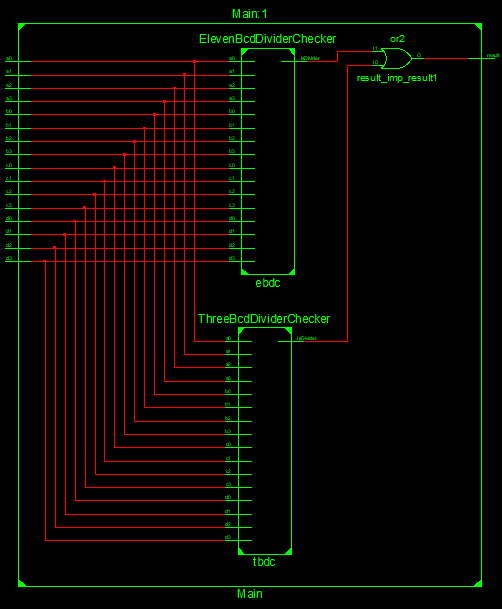
\includegraphics[width=.5\paperwidth]{./Schematic/Main.png}
	\caption{شماتیک ماژول اصلی}
	\label{main}
\end{figure}

\subsection{ماژول \lr{ElevenBcdDividerChecker}}
\begin{figure}[H]
	\centering
	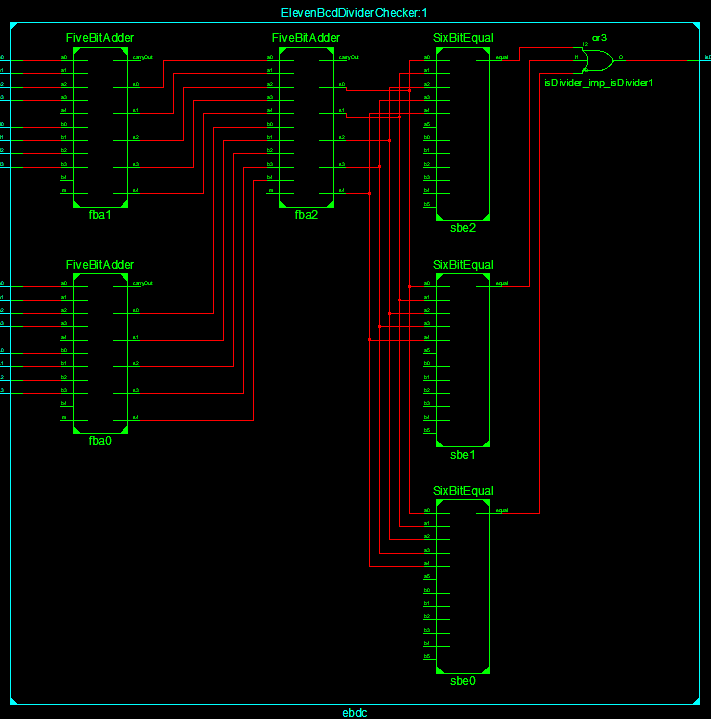
\includegraphics[width=.5\paperwidth]{./Schematic/EBDC.png}
	\caption{شماتیک ماژول بخش‌پذیری بر 11}
	\label{ebdc}
\end{figure}

\subsection{ماژول \lr{ThreeBcdDividerChecker}}
\begin{figure}[H]
	\centering
	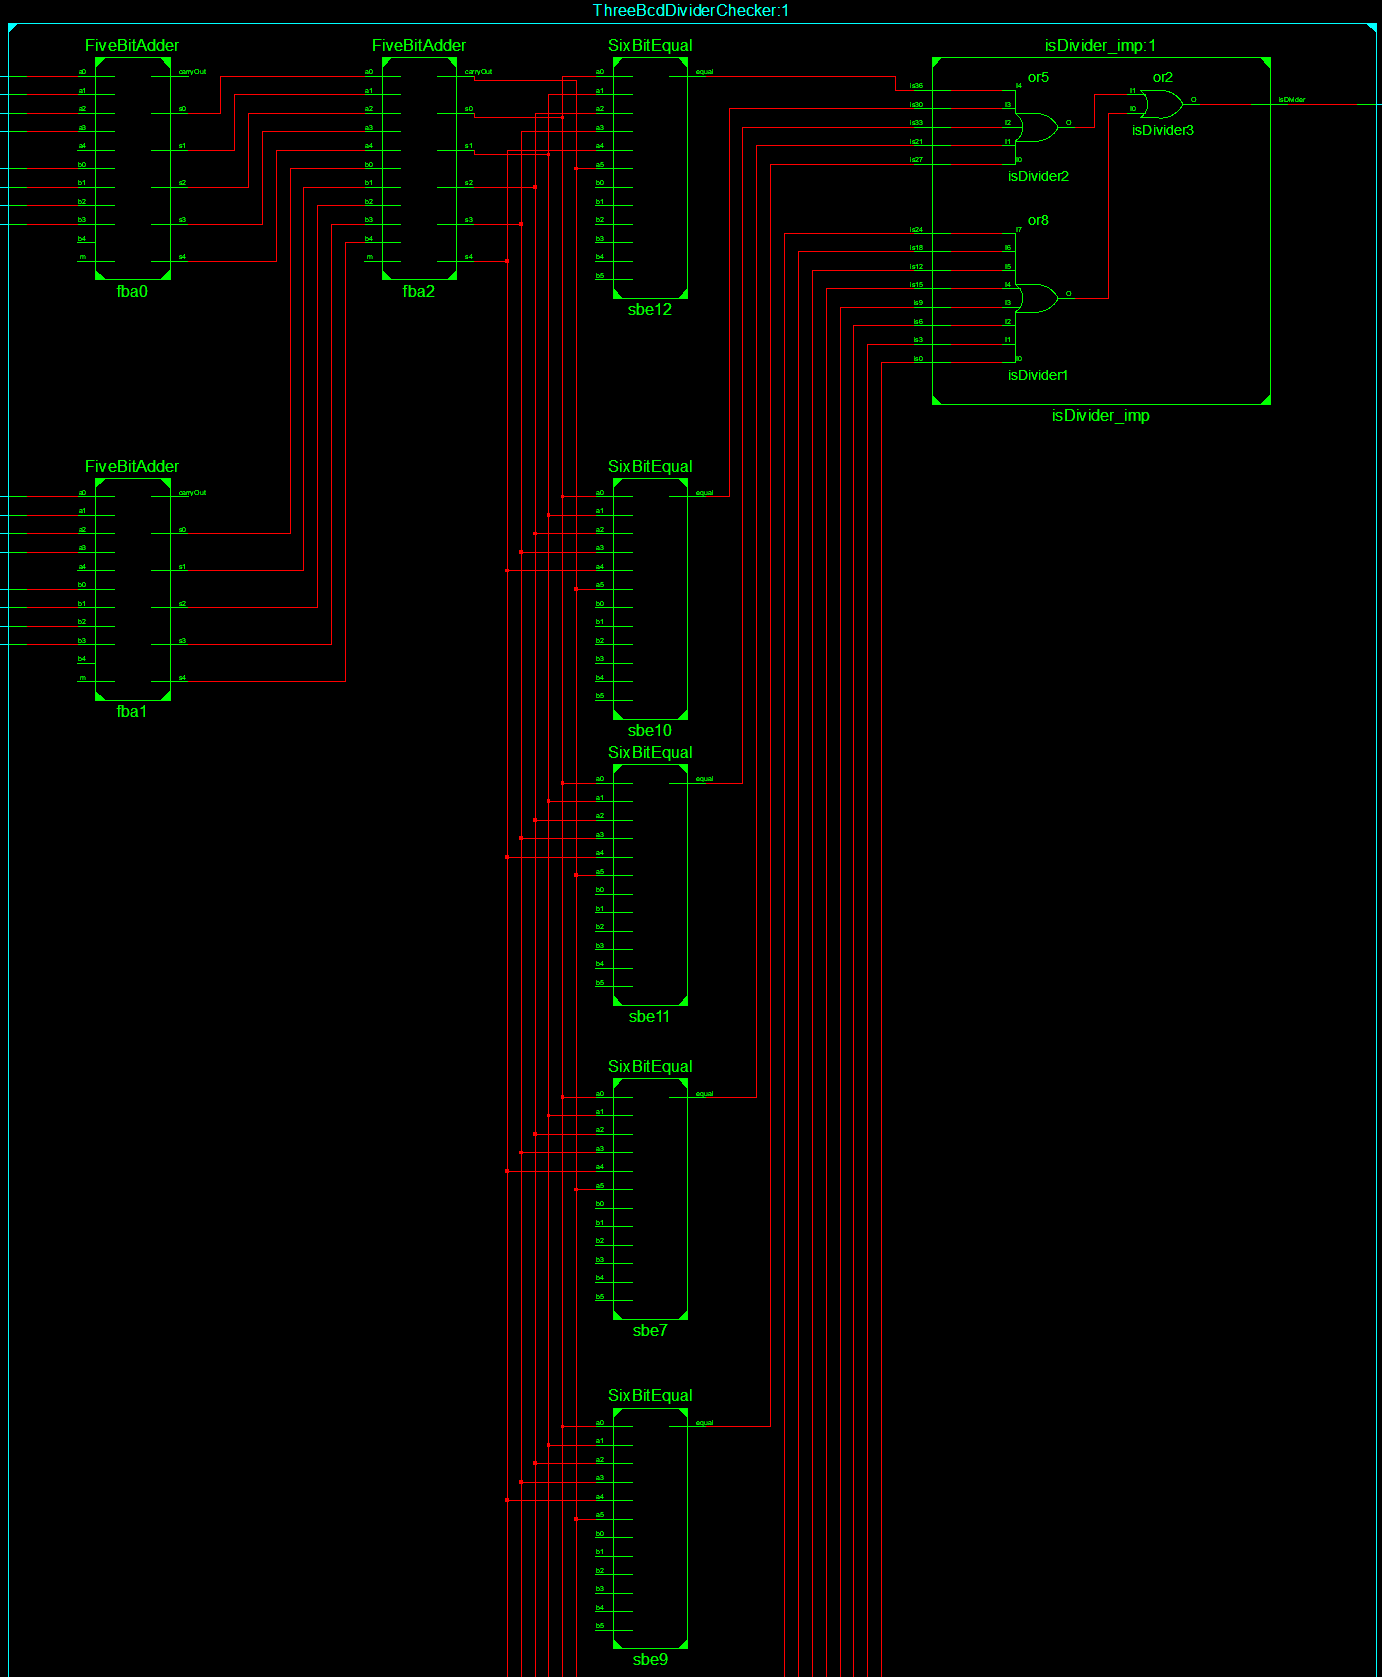
\includegraphics[width=.5\paperwidth]{./Schematic/TBDC1.png}
	\caption{شماتیک ماژول بخش‌پذیری بر 3 بخش 1}
	\label{tbdc31}
\end{figure}

\begin{figure}[H]
	\centering
	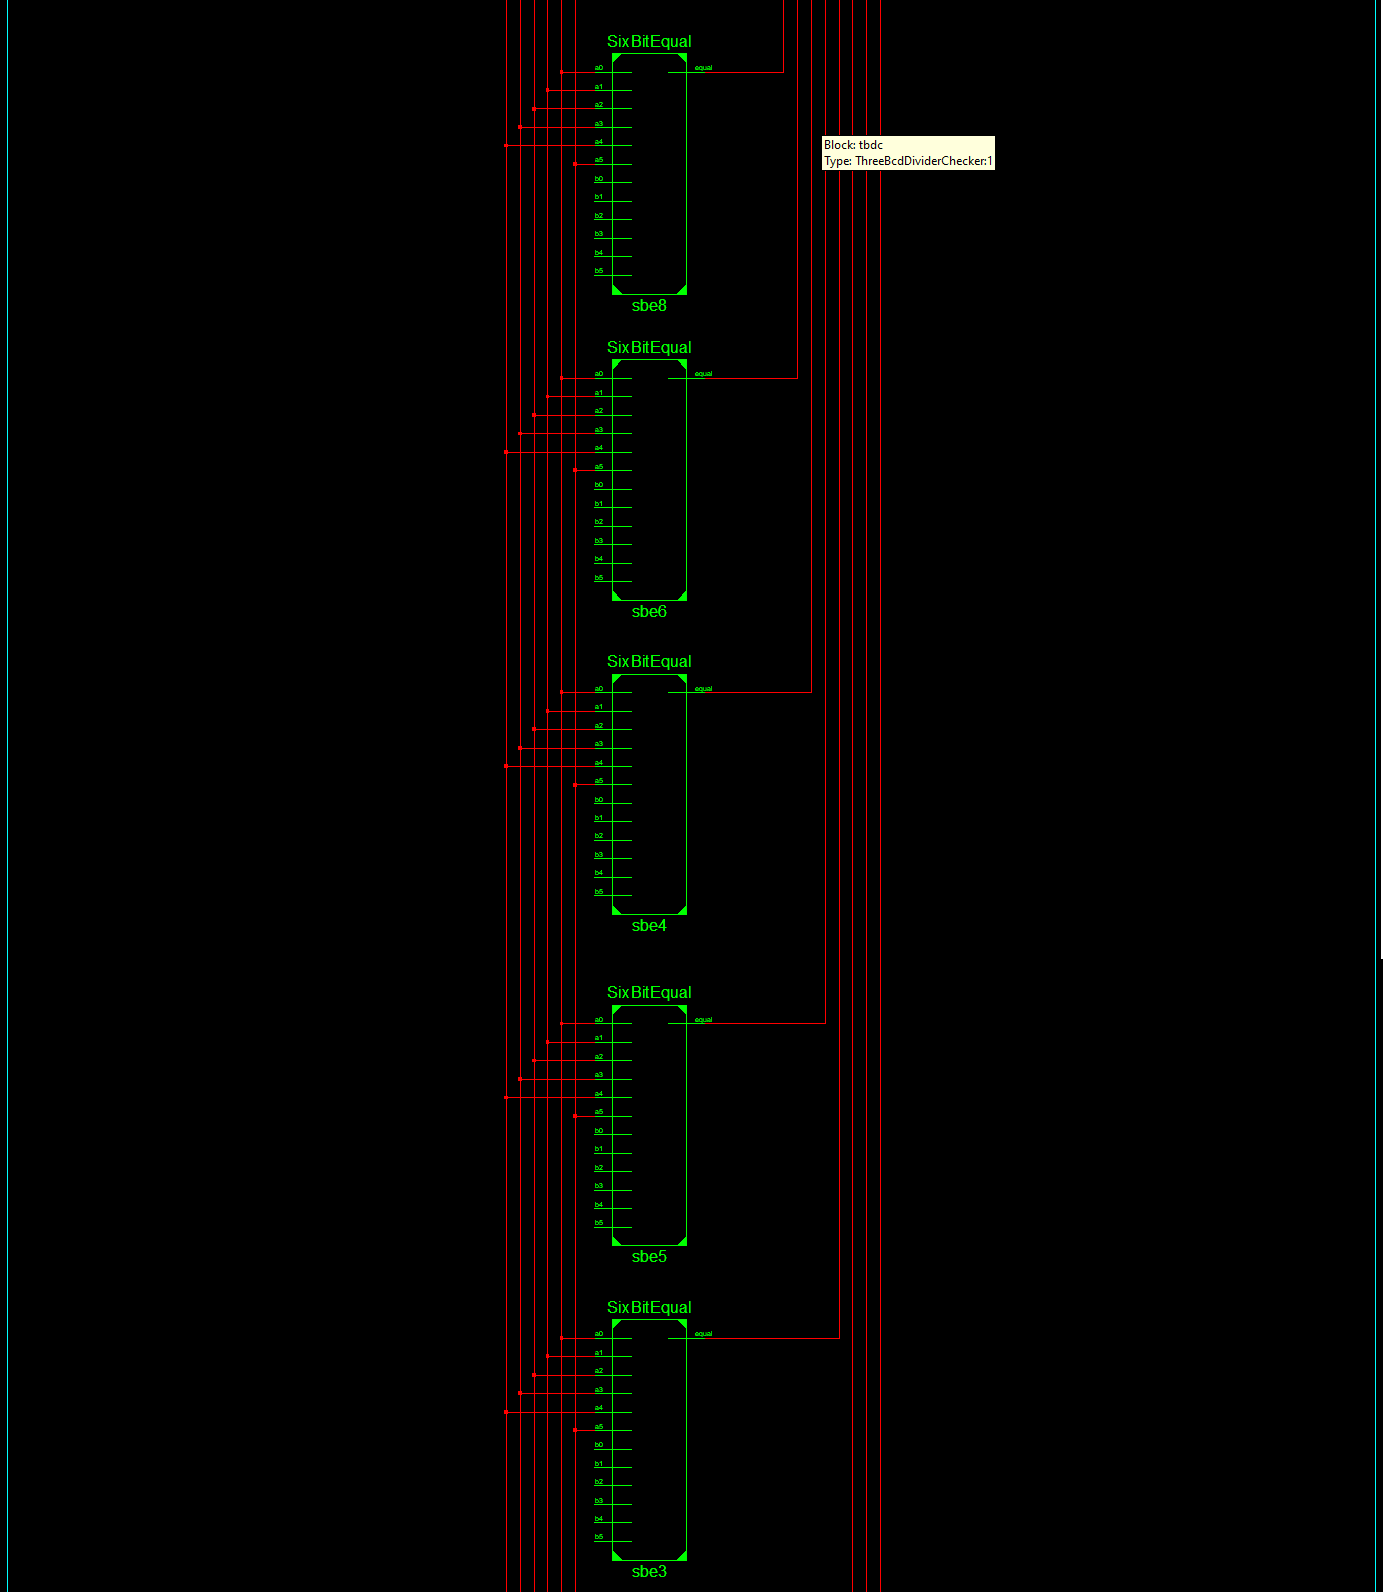
\includegraphics[width=.5\paperwidth]{./Schematic/TBDC2.png}
	\caption{شماتیک ماژول بخش‌پذیری بر 3 بخش 2}
	\label{tbdc32}
\end{figure}

\begin{figure}[H]
	\centering
	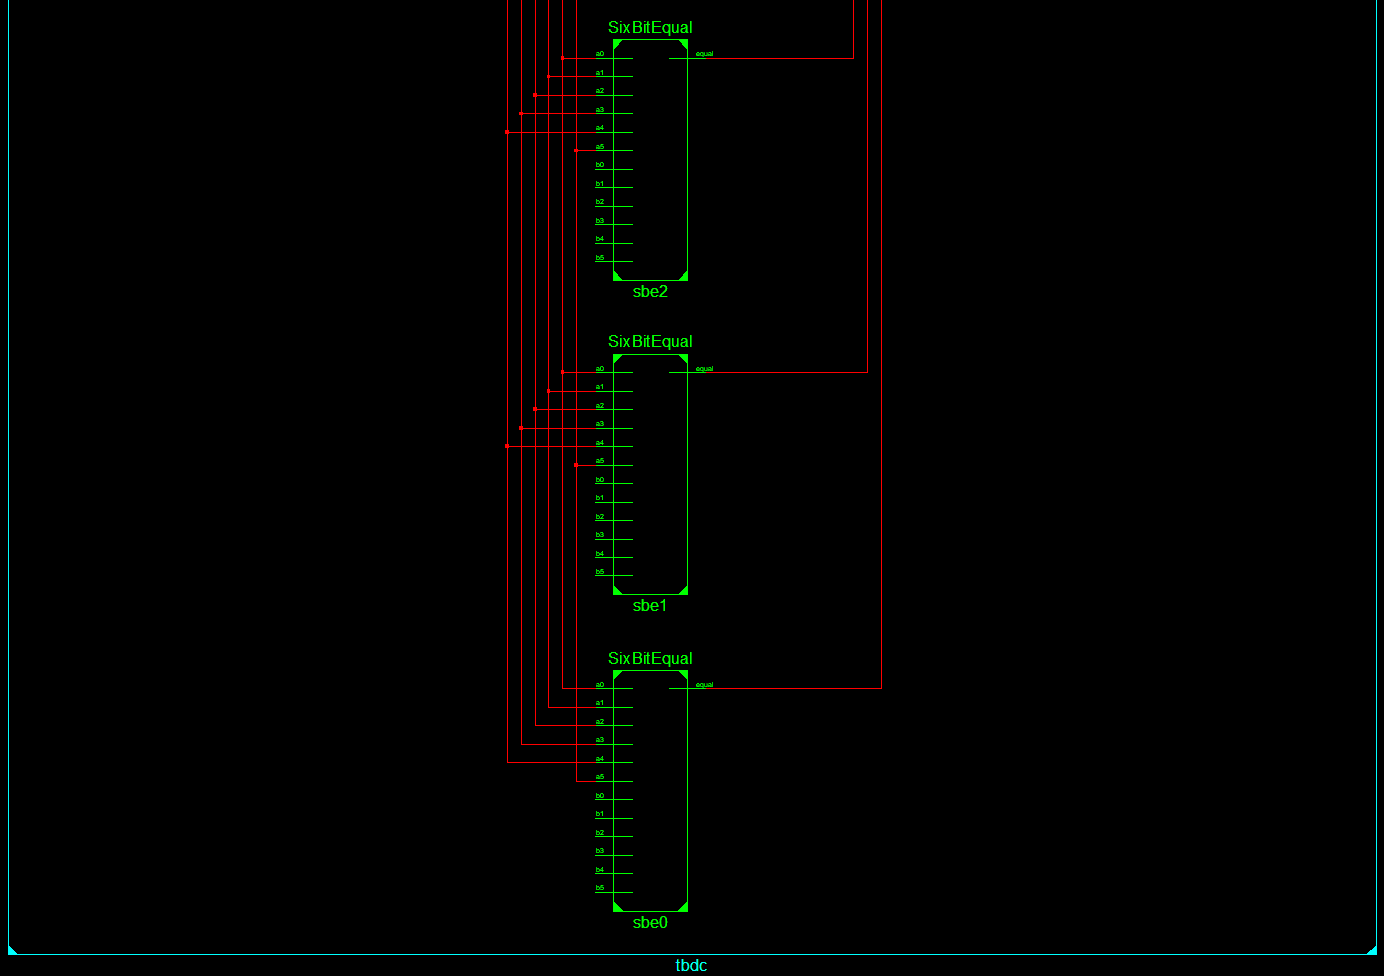
\includegraphics[width=.5\paperwidth]{./Schematic/TBDC3.png}
	\caption{شماتیک ماژول بخش‌پذیری بر 3 بخش 3}
	\label{tbdc33}
\end{figure}


\subsection{ماژول \lr{FiveBitAdder}}
\begin{figure}[H]
	\centering
	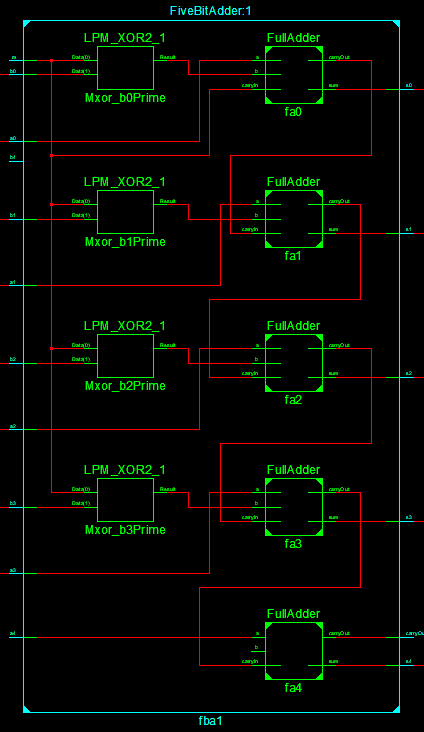
\includegraphics[width=.5\paperwidth]{./Schematic/FBA.png}
	\caption{شماتیک ماژول جمع/تفریق کننده 5 بیتی}
	\label{fba}
\end{figure}

\subsection{ماژول \lr{SixBitEqual}}
\begin{figure}[H]
	\centering
	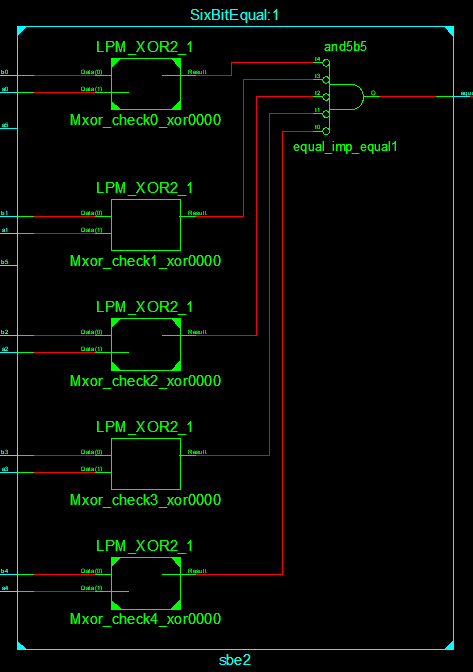
\includegraphics[width=.5\paperwidth]{./Schematic/SBE.png}
	\caption{شماتیک ماژول بررسی برابری دو عدد 6 بیتی}
	\label{sbe}
\end{figure}

\subsection{ماژول \lr{FullAdder}}
\begin{figure}[H]
	\centering
	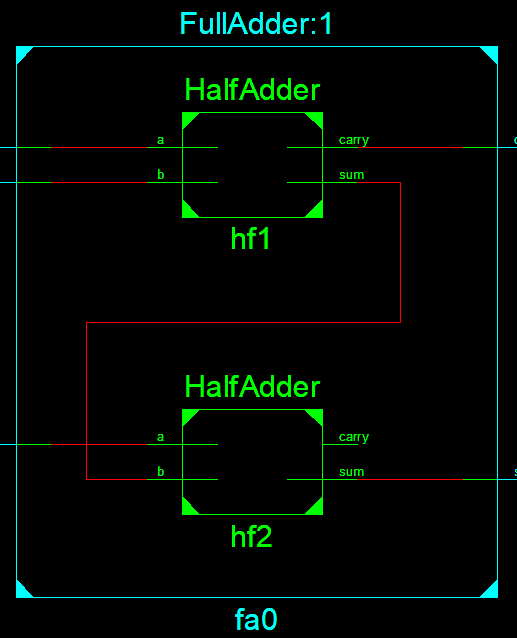
\includegraphics[width=.5\paperwidth]{./Schematic/FA.png}
	\caption{شماتیک ماژول جمع‌کننده کامل}
	\label{fa}
\end{figure}

\subsection{ماژول \lr{HalfAdder}}
\begin{figure}[H]
	\centering
	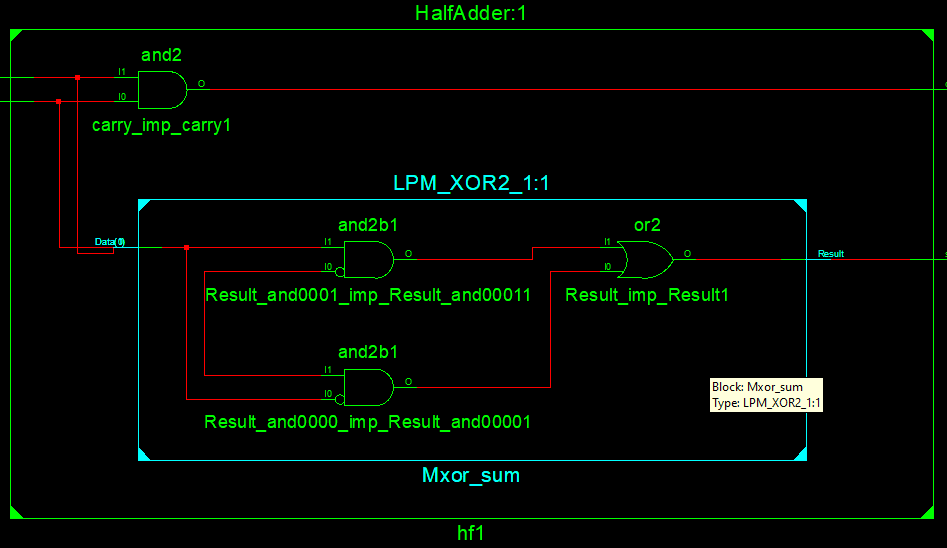
\includegraphics[width=.5\paperwidth]{./Schematic/HA.png}
	\caption{شماتیک ماژول نیم جمع‌کننده}
	\label{hf}
\end{figure}

\end{document}
